\section{HTM Recap}

\begin{frame}[c]{Biology}
    \Large
    \begin{itemize}[<+(1)->]
        \item The Neocortex is only a part of the brain
        \item The smallest computational units are called 'Cortical Columns'
        \item Every Neuron has on average 7'000 Connections 
    \end{itemize}
\end{frame}


\begin{frame}[c]{HTM Theory}
    \Large
    \begin{itemize}[<+(1)->]
        \item Biologically constrained, based on Neuroscience
        \item Everything is predicting everything
        \item Closest to how the brain really works
        \item Time is important
    \end{itemize}
\end{frame}


\begin{frame}[c]{Sparse Distributed Representation}
    \Large
    \begin{itemize}[<+(1)->]
        \item Data structure of the Brain
        \item Sparse (very few ON-bits)
        \item Distributed
        \item Required for other mechanisms
        \item Encoders are important!
    \end{itemize}
\end{frame}


\begin{frame}[c]{Learning}
    \Large
    \begin{itemize}[<+(1)->]
        \item Only statistical
        \item Based on Prediction and Inference
        \item Spatial and Temporal patterns
        \item Context sensitive
        \item Trying to minimize Errors (Bursting)
    \end{itemize}
\end{frame}


\begin{frame}[c]{Spatial Pooler}
    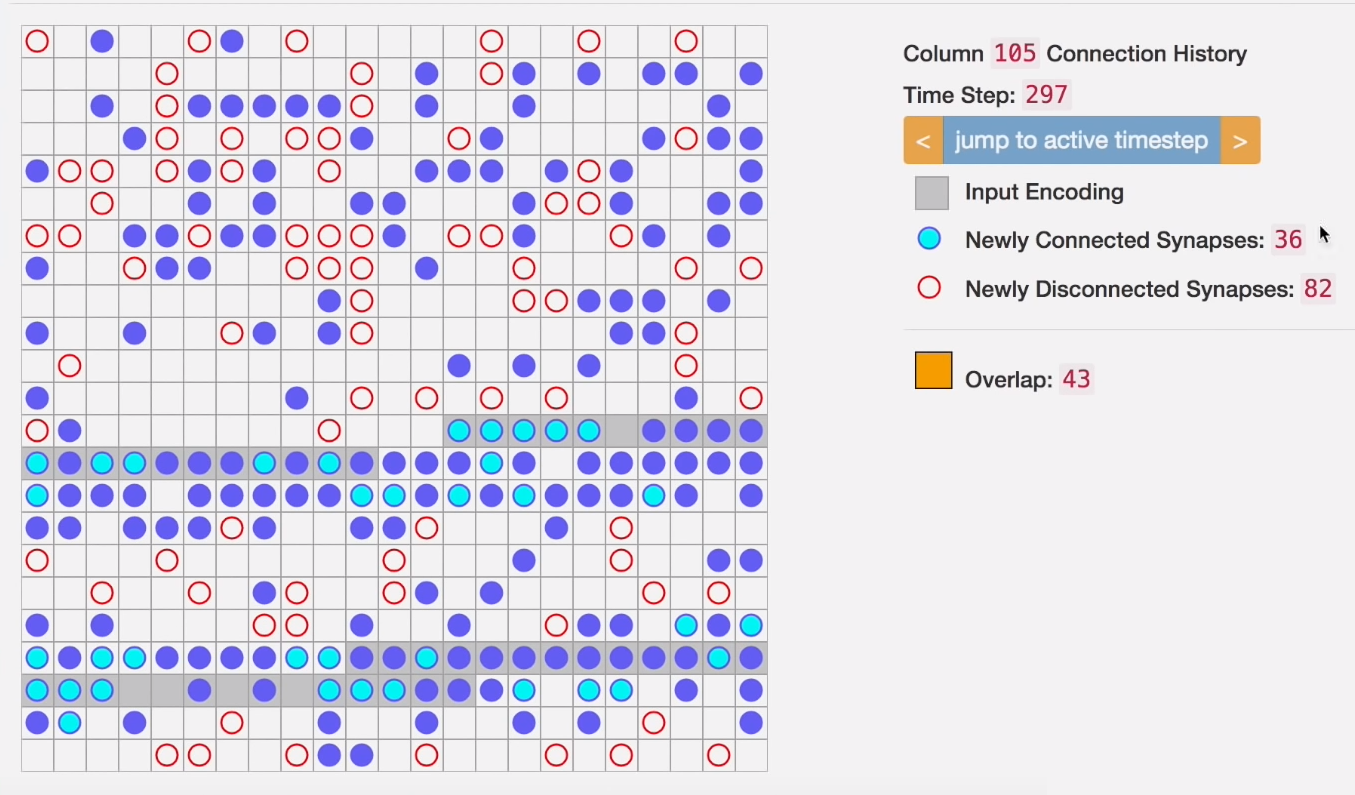
\includegraphics[width=\textwidth]{learn_ex2}
\end{frame}

\begin{frame}[c]{Spatial Pooler}
    \Large
    \begin{itemize}[<+(1)->]
        \item Calculate Overlap Scores (+Boosting)
        \item Inhibit
        \item Update connection values
    \end{itemize}
\end{frame}


\begin{frame}[c]{Temporal Pooler}
    \Large
    \begin{itemize}[<+(1)->]
        \item Form representations in context of previous states
        \item Form predictions based on previous inputs
        \item Context dependent
        \item Can modulate spatial pooler results
        \item One cell can represent many different concepts!
    \end{itemize}
\end{frame}





